%%%%%%%%%%%%%%%%%%%%%%%%%%%%%%%%%%%%%%%%%%%%%%%%%%%%%%%%%%%%%%%%%%%%%%%%%%%%%%%%
%2345678901234567890123456789012345678901234567890123456789012345678901234567890
%        1         2         3         4         5         6         7         8

\documentclass[letterpaper, 10 pt, conference]{ieeeconf}  % Comment this line out if you need a4paper

%\documentclass[a4paper, 10pt, conference]{ieeeconf}      % Use this line for a4 paper

\IEEEoverridecommandlockouts                              % This command is only needed if 
                                                          % you want to use the \thanks command

\overrideIEEEmargins                                      % Needed to meet printer requirements.

% See the \addtolength command later in the file to balance the column lengths
% on the last page of the document

% The following packages can be found on http:\\www.ctan.org
%\usepackage{graphics} % for pdf, bitmapped graphics files
%\usepackage{epsfig} % for postscript graphics files
%\usepackage{mathptmx} % assumes new font selection scheme installed
%\usepackage{times} % assumes new font selection scheme installed
%\usepackage{amsmath} % assumes amsmath package installed
%\usepackage{amssymb}  % assumes amsmath package installed
\usepackage{graphicx}
\usepackage[export]{adjustbox}
\usepackage{hyperref}
\graphicspath{ {images/} }


\title{\LARGE \bf
Multi-robot Patrolling with Multi-task
}


\author{Pin-Wei Chen$^{1}$% <-this % stops a space
\thanks{*This work was supported by the Robotics Master Program in National Chiao Tung University, Taiwan}% <-this % stops a space
\thanks{$^{1}$Pin-Wei Chen, National Chiao Tung University, Taiwan.		{\tt\small ccpwearth@gmail.com}}%
}


\begin{document}



\maketitle
\thispagestyle{empty}
\pagestyle{empty}


\section{INTRODUCTION \& MOTIVATION}

Multi-robot patrolling is an potential and practical project, we can apply this idea to surveillance, security, production line, etc. We realize that robot can help us with something routine and cycling. Just like patrolling, which we should patrol lots of nodes again and again. As a result, We come up with this idea, trying to build a multi-robot patrolling system in ROS, and also build this system base on duckietown. We will let the robots simulate the production line in factory. So the robots will reach specific node and do the specific task, such as grabbing things or press the botton.

\section{SYSTEM ARCHITECTURE \& EQUIPMENTS}

\subsection{SYSTEM ARCHITECTURE}

We will have one master robot (Raspberry Pi3) and lots of patrolling robots (duckiebots). The master and all of the robots are all connected to the same router, so that the master can communicate with each robot.

Each robot will follow the yellow line, and when they arrive at the patrolling node, they will stop and wait for the order from the master. The master will tell the robot to go straight or turn back as each robot arrived at the patrolling node Fig.~\ref{figure:chart}.
\begin{figure}[h] % t means put this image at the top 
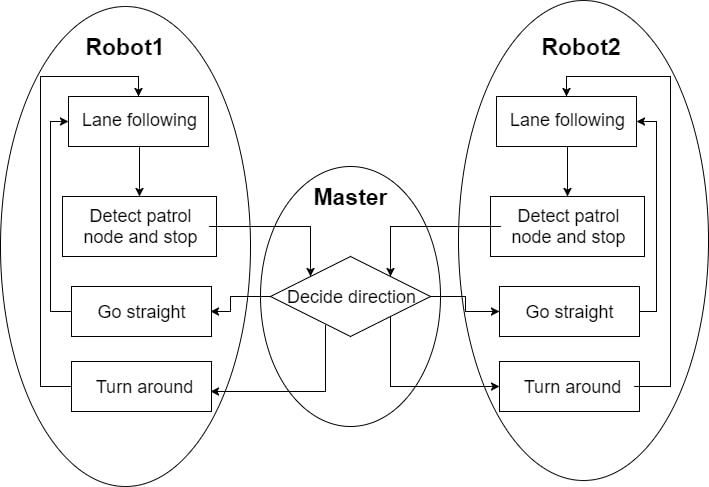
\includegraphics[width=0.8\columnwidth]{flowchart}
\centering
\caption{Multi-robot patrolling flowchart}
\label{figure:chart}
\end{figure}

\subsection{EQUIPMENTS} 

The patrolling robots we use are Moified from duckiebots, we replace the dagu motor with JGB37-520 motor, which have an encoder in it. In addition, we use yellow lines and black background as our patrolling map, and we use apriltags as the patrolling nodes Fig.~\ref{figure:map}. In software part, we use ROS kinetic and ubuntu 16.04 LTS as our develop enviromnet.

\begin{figure}[t] % t means put this image at the top 
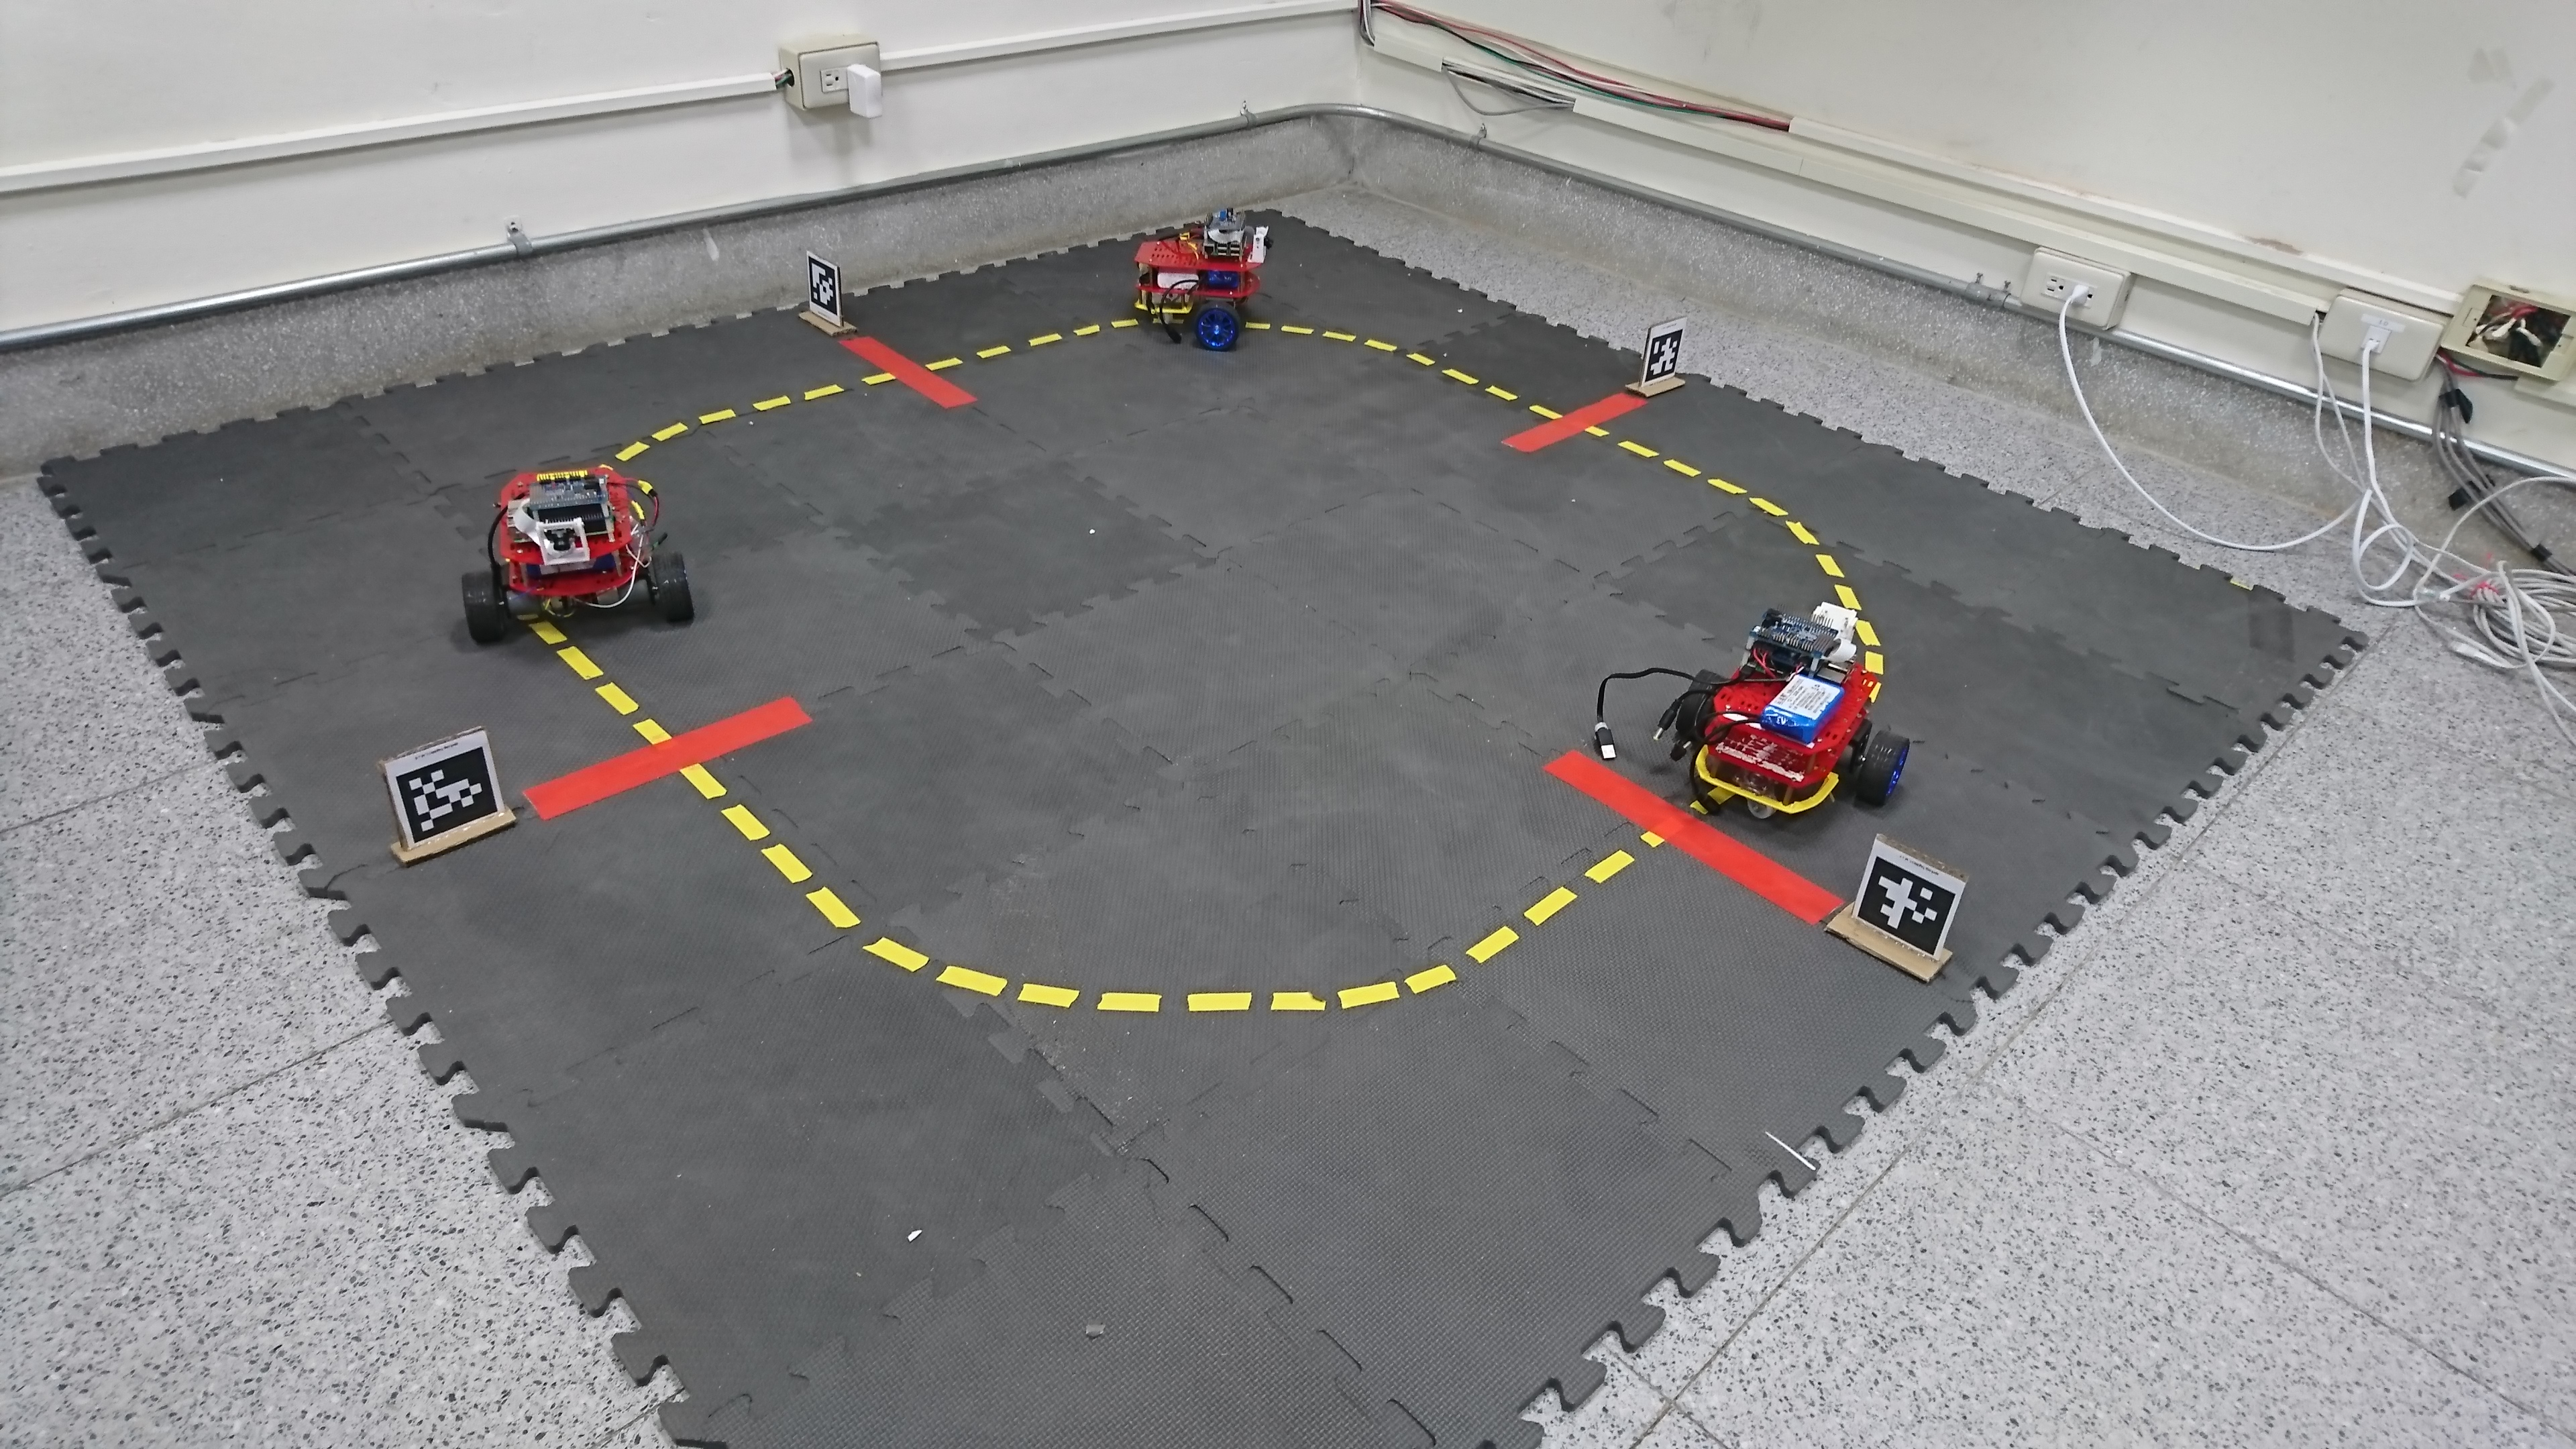
\includegraphics[width=1\columnwidth]{map}
\centering
\caption{Multi-robot patrolling map}
\label{figure:map}
\end{figure}

\section{SPECIFIC AIMS}

\begin{itemize}
\item Patrolling multi-node
\end{itemize}
We are trying to let the robot patrol multi-node, and each node will be patrolled in approximately the same idle time.
\begin{itemize}
\item Arrive specific patrolling node and avoid obstacles
\end{itemize}
when the robot is going to visit specific patrolling node, and there are some obstacles floating between the robot and goal, the robot should detect where the obstacles are and autumatically avoid it.
\begin{itemize}
\item Multi-robot patrolling
\end{itemize}
We will let multi-robot patrol multi-node, in addition to that each node will have same idleness, those robot will not patrol on the same lane at the same time, or they will crash with each other.
We will build a virtual world and models in Gazebo, and try to move all of 
\begin{itemize}
\item Patrolling with multi-task
\end{itemize}
As the robot arrive specific patrolling node, it will do the corresponding task, such as grabbing object or press the botton. This situation is simulate the production line in the real factory.

\section{APPROACH}

We will modify the lane following in duckietown, and let the robots can patrol along the yellow line. And we will use apriltags with different ID to let the robot know which node they are patrolling now, it's kind of locating the robot.

The algorithm I use is refer to "Distributed On-line Dynamic Task Assignment for Multi-robot Patrolling"~\cite{Farinelli:2017:DOD:3124264.3124274}, we will measure the idleness of each node first, and than the master will coordinate every robot to let the nodes with larger idleness be patrolled first. If any node is going to be patrolled, the idleness will return to zero, so that no two robots will go to the same node at the same time, and it can avoid collision.   


\section{SCHEDULE AND TEAM COLLABORATION}

I expect this project can finish real world patrolling before November, and can excute in Gazebo before December. The experiment video is available in this link: \url{https://goo.gl/sDwa9j}.

\addtolength{\textheight}{-12cm}   % This command serves to balance the column lengths
                                  % on the last page of the document manually. It shortens
                                  % the textheight of the last page by a suitable amount.
                                  % This command does not take effect until the next page
                                  % so it should come on the page before the last. Make
                                  % sure that you do not shorten the textheight too much.

\bibliographystyle{IEEEtran}
\bibliography{egbib}

\end{document}
